\documentclass{article}
\usepackage{times}
\usepackage{graphicx}
\usepackage{subfigure} 
\usepackage{natbib}
\usepackage{algorithm}
\usepackage{algorithmic}
\usepackage{hyperref}
\newcommand{\theHalgorithm}{\arabic{algorithm}}
\usepackage[accepted]{icml2017}
\usepackage{lipsum}
\usepackage{tikz}
\newcommand{\mycbox}[1]{\tikz{\path[draw=#1,fill=#1] (0,0) rectangle (0.2cm,0.2cm);}}
\usepackage{amsmath}
\usepackage[noend]{algpseudocode}
\usepackage[usenames, dvipsnames]{color}
\documentclass[usenames,dvipsnames]{beamer}
\usepackage{biblatex}
\addbibresource{references.bib}

\icmltitlerunning{Variance Reduction for Low Precision Arithmetic}

\begin{document} 

\twocolumn[
\icmltitle{CS 6787 Project : 
           Variance Reduction for Low Precision Arithmetic}

\icmlsetsymbol{equal}{*}

\begin{icmlauthorlist}
\icmlauthor{Abigail Shchur (aks236)}{equal,cornell}
\icmlauthor{Sergio Palomo (sdp85)}{equal,cornell}
\icmlauthor{Serena Li (sl2327)}{equal,cornell}
\end{icmlauthorlist}

\icmlaffiliation{cornell}{Cornell University, USA}
\icmlcorrespondingauthor{Abigail Shchur}{aks236@cornell.edu}
\icmlcorrespondingauthor{Sergio Palomo}{sdp85@cornell.edu}
\icmlcorrespondingauthor{Serena Li}{sl2327@cornell.edu}


\icmlkeywords{HALP}

\vskip 0.2in
]

%\printAffiliationsAndNotice{\icmlEqualContribution} % otherwise use the standard text.

\begin{abstract}
Training using Stochastic Gradient Descent (SGD) is often heavily constrained due to limited computational resources. This bottleneck can be mitigated by utilizing low precision arithmetic which is known to decrease energy consumption and improve throughput. However, naively using low precision representations can slow down convergence and result in a low accuracy model. This is because the loss of information from the quantization steps that are necessary to maintain a low precision model can be seen as a form variance. We evaluate the effect of combining low precision arithmetic with SVRG on Linear Regression and Matrix Completion. Specifically, we look at the convergence rate of a naive implementation of Low Precision SVRG (LP-SVRG). We also evaluate the convergence rate of High Accuracy Low Precision SVRG (HALP) - an algorithm that uses full precision weights but low precision weight updates. Lastly we evaluate the convergence rate and speedup from an optimized version of LP-SVRG for linear models. We found that implementing LP-SVRG in a way that outperforms full precision SVRG in terms of wallclock time is not feasible given the limitations of Numpy arrays in Python. However, the empirical analysis of convergence rates verified that low precision implementations of SVRG are comparable to their full precision counterparts. 
\end{abstract} 

\section{Introduction}
In this report, we empirically evaluate low precision variants of SVRG \cite{Johnson:2013:ASG:2999611.2999647}. We begin by limiting our scope to linear regression. The first algorithm we evaluate is LP-SVRG-LR which is an implementation of low precision SVRG for linear regression where weights are stored using low precision representations and weight updates are quantized \cite{Gupta:2015:DLL:3045118.3045303}. We then evaluate LP-SVRG-LR-OPT which is a low precision SVRG algorithm for linear regression that is optimized for speed. Then, we look at HALP-LR \cite{halp} which is a high accuracy method of low precision SVRG. These algorithms are evaluated by looking at their error rates and wallclock times for all calculations after each epoch. Next, we implement the LP-SVRG and HALP algorithms for matrix completion. Here, we only focus on seeing how convergence rates differ. 

A particular low precision representation is denoted using a color, scale factor, and number of bits. Concretely, we say that $\mycbox{blue} = (\delta,b)$ means that the ``blue" numbers are represented using $b$ bits and they have a scale factor of $\delta$. If we want to represent numbers from roughly -1 to 1, we could set $\delta = \frac{1}{2^{b-1}}$ for any $b$. To perform quantization, we say that $Q_{\mycbox{blue}}(x)$ converts a floating point representation of $x$ to the \mycbox{blue} low precision representation. The quantization function always uses saturating arithmetic and stochastic rounding. It is important to note that when using a low precision representation of the model, the accuracy of the result from any optimization algorithm will not be better than that of the best possible model given that low precision representation.
\section{Linear Regression} 
The theoretical results for the algorithms discussed in this report show that we can maintain the linear converge rate of SVRG for strongly convex loss functions when using low precision representations. To verify this, we began by implementing the algorithms for linear regression. Essentially, we want to solve the following optimization problem using a squared loss function: 

\begin{equation}min \ f(w) = \frac{1}{n}\sum_{i=1}^n l(w^T x_i)\end{equation}
\subsection*{Low Precision LR}
Implementing a low precision variant of SVRG for linear regression is fairly straightforward. First, we choose a low precision representation for the weights. Then, we run SVRG for linear regression normally except we add a quantization step before the inner loop weight update.


\begin{algorithm}[H]
\caption{LP-SVRG-LR}
\begin{algorithmic}
   \STATE {\textbf{given:}} number of epochs $K$, epoch length $T$, step size $\alpha$, initial iterate $\color{blue}w_{0,T}$
   \STATE {\textbf{given:}} low-precision representation $\mycbox{blue} = (\delta, b)$
   \FOR
   {$k=1, 2, ..., K$}
   \STATE $\color{blue}\tilde{w}_k \color{black}\leftarrow \color{blue}w_{k-1,T}$
   \STATE $\tilde{g}_k \leftarrow \bigtriangledown f (\color{blue} \tilde{w}_k \color{black}) = \frac{1}{n}\sum_{i=1}^n \bigtriangledown f_i (\color{blue} \tilde{w}_k \color{black})$
   \STATE $\color{blue}w_{k,0} \color{black} \leftarrow \color{blue} \tilde{w}_k $
   \FOR
   {$t=1, 2, ... ,T$}
   \STATE sample $i$ uniformly from \{$1,...,N$\}
   \STATE $\color{blue}w_{k,t} \color{black} \leftarrow Q_{\mycbox{blue}}(\color{blue} w_{k,t-1} \color{black} - \alpha (\bigtriangledown f_i (\color{blue} w_{k,t-1} \color{black}) - \bigtriangledown f_i (\color{blue} \tilde{w}_k \color{black}) + \tilde{g}_k)) $
   \ENDFOR \ENDFOR
   \RETURN $\color{blue} w_{K,T}$\color{white}
\end{algorithmic}
\end{algorithm}

\subsection*{Optimized Low Precision SVRG for LR}
To implement a version of LP-SVRG-LR that is optimized for speed, we first assume that we have a low precision representation of our data (\mycbox{red}). We also define a low precision representation of our weights (\mycbox{blue}). The goal of this implementation is to only use low precision arithmetic in the inner loop gradient update. To accomplish this, we can define intermediate representations \mycbox{green} and \mycbox{violet} as shown in the pseudo-code for LP-SVRG-LR-OPT.  
\begin{algorithm}[H]
\caption{LP-SVRG-LR-OPT}
\begin{algorithmic}
   \STATE {\textbf{given:}} number of epochs $K$, epoch length $T$, step size $\alpha$, initial iterate $\color{blue} w_{0,T}$
   \STATE {\textbf{given:}} low-precision model representation $\mycbox{blue}$
   \STATE {\textbf{given:}} low-precision data representation $\mycbox{red}$
   \STATE {\textbf{given:}} low-precision intermediate representation $\mycbox{violet}$
   \STATE {\textbf{given:}} low-precision intermediate representation $\mycbox{green} = \mycbox{red} \times \mycbox{violet}$
   \FOR
   {$k=1, 2, ..., K$}
   \STATE $\color{blue}\tilde{w}_k \color{black}\leftarrow \color{blue}w_{k-1,T}$
   \STATE $\color{green}\tilde{h}_k \color{black} \leftarrow  Q_{\mycbox{green}} (\frac{\alpha}{n}\sum_{i=1}^n l_i'(\color{red}x_i^{\color{black}T}\color{blue}\tilde{w}_k \color{black})\color{red}x_i\color{black})$
   \STATE $\color{blue}w_{k,0} \color{black} \leftarrow \color{blue} \tilde{w}_k $
   \FOR
   {$t=1, 2, ... ,T$}
   \STATE sample $i$ uniformly from \{$1,...,N$\}
   \STATE $\color{blue}w_{k,t} \color{black} \leftarrow Q_{\mycbox{blue}}(\color{blue} w_{k,t-1} \color{black} - Q_{\mycbox{violet}} \color{black} (l_i'(\color{red}x_i^{\color{black}T}\color{blue}w_{k,t-1}\color{black}) - l_i' (\color{red} x_i^{ \color{black}T} \color{blue} \tilde{w}_k \color{black})))\color{red} x_i \color{black} - \color{green} \tilde{h}_k\color{black}) $
   \ENDFOR \ENDFOR
   \RETURN $\color{blue} w_{K,T}$\color{white}
\end{algorithmic}
\end{algorithm}

\subsection*{High Accuracy Low Precision SVRG for LR}
To implement High Accuracy Low Precision SVRG, we store full precision weights but we make low precision weight updates. Intuitively, this algorithm does something similar to running LP-SVRG-LR, saving the result in a high precision weight vector, and then running LP-SVRG-LR again to fine tune that weight vector. This is done by storing a low precision weight update and updating the scale factor for the low precision weight update after each epoch. To re-scale the scale factor, the algorithm does require a hyper-parameter $\mu$. From a theoretical standpoint, $\mu$ is the strong convexity constant for a given loss function. Although it can be explicitly calculated for linear regression, we chose to treat it as a proper hyper-parameter and tuned it using grid search. 
\begin{algorithm}[H]
\caption{HALP-LR}
\begin{algorithmic}
   \STATE {\textbf{given:}} number of epochs $K$, epoch length $T$, step size $\alpha$, initial iterate $w_{0,T}$
   \STATE {\textbf{given:}} number of low precision bits $b$
   \STATE $\color{blue} z_{0,T} \color{black} \leftarrow \color{blue} 0$
   \FOR
   {$k=1, 2, ..., K$}
   \STATE $\tilde{w}_k \leftarrow w_{k-1} + \color{blue} z_{k-1,T}$
   \STATE $\tilde{g}_k \leftarrow \bigtriangledown f (\tilde{w}_k) = \frac{1}{n}\sum_{i=1}^n \bigtriangledown f_i (\tilde{w}_k)$
   \STATE $s_k \leftarrow \frac{||\tilde{g}_k||}{\mu (2^{b-1}-1)}$
   \STATE {\textbf{re-scale:}} $\mycbox{blue} = (s_k, b)$
   \STATE $\color{blue}z_{k,0} \color{black} \leftarrow \color{blue}0 $
   \FOR
   {$t=1, 2, ... ,T$}
   \STATE sample $i$ uniformly from \{$1,...,N$\}
   \STATE $\color{blue}z_{k,t} \color{black} \leftarrow Q_{\mycbox{blue}}(\color{blue} z_{k,t-1} \color{black} - \alpha (\bigtriangledown f_i (\tilde{w}_k + \color{blue} z_{k,t-1} \color{black}) - \bigtriangledown f_i (\tilde{w}_k) + \tilde{g}_k)) $
   \ENDFOR \ENDFOR
   \RETURN $\tilde{w}_{K,T} + \color{blue} z_{K,T}$\color{white}
\end{algorithmic}
\end{algorithm}

\section{Linear Regression Experiments}

To evaluate the preceding algorithms, we generated an artificial dataset ($X$) of 10,000 points with 100 dimensions where each entry was independently sampled uniformly from the numbers that can be represented using 8 bits with a scale factor of $\frac{1}{2^{8-1}}$. In other words, the float value of each data point was between -1 and 1 but we enforced a low precision representation. The ground truth weights were chosen uniformly from -1 to 1 using full precision. The ground truth labels ($Y$) were calculated using the dot product of the weights and the data points. Some noise was also added. In addition, we consistently used a step size of 0.001, 20 total epochs, and an epoch length of $1000$. The same random weight initialization is also used for all tests. For cases where weights are low precision, we simply quantize the random initialization. All code was written in Python and we attempted to take advantage of speedups from using low precision Numpy arrays for dot products. 

We began by implementing a version of full precision SVRG for linear regression to compare the other algorithms to. Then, implementing LP-SVRG-LR was fairly straightforward. We chose a $\mycbox{blue} = (\frac{1}{2^{8-1}}, 8)$ representation for the weights. 

Implementing LP-SVRG-LR-OPT was a bit more involved due to the ambiguity in how we can choose the low precision representations. The representation of the data ($X$) is set in stone to be $\mycbox{red} = (\frac{1}{2^{8-1}}, 8)$ since that is how we generated the data. The other colors can however be initialized in different ways. Since we know that the weights truly range from -1 to 1, there were only two reasonable choices for how to assign the colors. One option was $\mycbox{blue} = (\frac{1}{2^{16-1}}, 16)$, $\mycbox{green} = (\frac{1}{2^{16-1}}, 16)$, $\mycbox{violet} = (\frac{\delta_{green}}{\delta_{red}}, 8)$. The other option was $\mycbox{blue} = (\frac{1}{2^{8-1}}, 8)$, $\mycbox{green} = (\frac{1}{2^{16-1}}, 16)$, $\mycbox{violet} = (\frac{\delta_{green}}{\delta_{red}}, 8)$. In both settings, we observed that the expressivity of the  $\mycbox{violet}$ quantization section limited the accuracy of the algorithm. When the weights are 16 bits, we see that the error rate decreases but at a significantly slower rate than SVRG. When the weights are 8 bit, the algorithm does not converge because the $\mycbox{violet}$ quantization sets most values to 0. Interestingly, if we multiply by $\alpha$ after the $\mycbox{violet}$ quantization, the algorithm converges to the same point as LP-SVRG-LR (this is what we show in the plot below). Unfortunately, this creates a situation where you need to do more full precision arithmetic within the inner loop. 

HALP is a fairly straightforward algorithm to implement. We first tried to use 8 bit weight updates but that did not converge for any setting of $\mu$. When using 16 bit weight updates, the algorithm does converge. In fact, the convergence rate curve looks almost equivalent to that of full precision SVRG. INSERT SOMETHING ABOUT HOW WE CHOSE MU FOR THE OPTIMAL ONE. 

\begin{figure}[ht!]
    \centering
    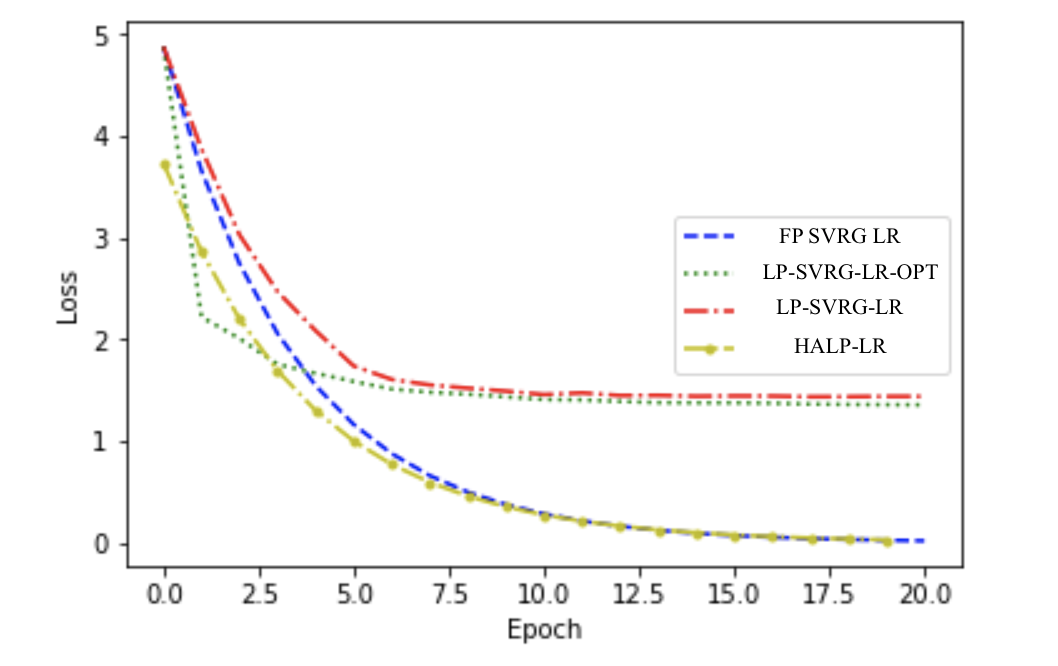
\includegraphics[width=.5\textwidth]{pic3.png}
\end{figure}

One interesting observation from the plot above is that the both LP-SVRG-LR-OPT and HALP-LR initially have steeper drops in error than full precision SVRG. 

INSERT STUFF ABOUT RUNTIME HERE

\section{Matrix Completion}
The matrix completion problem is easily framed in the context of the Netflix problem. Let $\mathbf{R}$ of size $|U| \times |D|$ be the matrix that contains all the ratings that the users have assigned to the items, where U is a set of users, and a D is a set of movies. Also, we assume that we would like to discover $K$ latent features. Our task, then, is to find two matrices $\mathbf{P}$ (a $|U| \times K$ matrix) and $\mathbf{Q}$ (a $|D| \times K$ matrix) such that their product approximates $\mathbf{R}$:
\begin{equation}
\mathbf{R} \approx \mathbf{P} \times \mathbf{Q}^T = \hat{\mathbf{R}}
\end{equation}

Each row of $\mathbf{P}$ would represent the strength of the associations between a user and the features. Similarly, each row of $\mathbf{Q}$ would represent the strength of the associations between an item and the features. To get the prediction of a rating of an item $d_j$ by $u_i$, we can calculate the dot product of the two vectors corresponding to $u_i$ and $d_j$:
\begin{equation}
\hat{r}_{ij} = p_i^T q_j = \sum_{k=1}^k{p_{ik}q_{kj}}
\end{equation}

Now, we have to find a way to obtain $\mathbf{P}$ and $\mathbf{Q}$. One way to approach this problem is the first initialize the two matrices with some values, calculate how `different’ their product is to $\mathbf{M}$, and then try to minimize this difference iteratively. Such a method is called gradient descent, aiming at finding a local minimum of the difference. The difference here, usually called the error between the estimated rating and the real rating, can be calculated by the following equation for each user-item pair:

\begin{equation}
e_{ij}^2 = (r_{ij} - \hat{r}_{ij})^2 = (r_{ij} - \sum_{k=1}^K{p_{ik}q_{kj}})^2
\end{equation}

Here we consider the squared error because the estimated rating can be either higher or lower than the real rating.
To minimize the error, we have to know in which direction we have to modify the values of  $p_{ik}$ and $q_{kj}$. In other words, we need to know the gradient at the current values, and therefore we differentiate the above equation with respect to these two variables separately:
\begin{align*} 
\frac{\partial}{\partial p_{ik}}e_{ij}^2  &= -2(r_{ij} - \hat{r}_{ij})(q_{kj}) \\
\frac{\partial}{\partial q_{ik}}e_{ij}^2  &= -2(r_{ij} - \hat{r}_{ij})(p_{ik}) 
\end{align*}

Having obtained the gradient, we can now formulate the update rules for both $p_{ik}$ and $q_{kj}$:
\begin{align*}
p'_{ik} &= p_{ik} + \alpha \frac{\partial}{\partial p_{ik}}e_{ij}^2  \\ 
q'_{kj} &=  q_{kj} + \alpha \frac{\partial}{\partial q_{kj}}e_{ij}^2  
\end{align*}

Below are the algorithms presented in the High Accuracy SGD with Low Precision Arithmetic Using Variance Reduction write up modified for matrix completion.  

\subsection*{Matrix Completion HP-SVRG}
\begin{algorithm}[H]
   \caption{Matrix Completion HP-SVRG}
   \label{alg:example}
\begin{algorithmic}
   \STATE {\bfseries Input:} m (update frequency), $\eta$(learning rate)
   \STATE {\bfseries Initialize:} $\mathbf{P}_0, \mathbf{Q}_0$
   %\STATE {\bfseries Iterate:} for s =1,2, ...
   %\REPEAT
   %\STATE Initialize $noChange = true$. \mycbox{red} 
   \FOR{$s=1, 2, ...$}
   \STATE $\Tilde{\mathbf{P}} = \Tilde{\mathbf{P}}_{s-1}$
   \STATE $\Tilde{\mu}_P = \frac{1}{n} \sum_{i=1}^n \nabla \psi_i (\Tilde{P})$
   \STATE $\mathbf{P}_0 = \Tilde{P}, \mathbf{Q}_0 = \Tilde{Q}$
   \FOR{$t=1, 2, ...$}
   \STATE Randomly pick index $i_t $and update weight
   \STATE $\mathbf{P}_t = \mathbf{P}_{t-1} -\eta (\nabla \psi_{i_t}(\mathbf{P}_{t-1}) - \nabla \psi_{i_t}(\Tilde{\mathbf{P}}))$
   \ENDFOR
   \STATE set $\Tilde{\mathbf{P}}_s = \mathbf{P}_m $
   \ENDFOR
   \color{white}
\end{algorithmic}
\end{algorithm}

\subsection*{Matrix Completion LP-SVRG}

Algorithm is supposed to be here.
\begin{algorithm}[H]
   \caption{Matrix Completion LP-SVRG}
   \label{alg:example}
\begin{algorithmic}
   \STATE {\bfseries Input:} m (update frequency), $\eta$ (learning rate), 
   \STATE {\bfseries Input:} low precision representation $\mycbox{blue} = (\delta,b)$
   \STATE {\bfseries Initialize:} $\mathbf{P}_0, \mathbf{Q}_0$
   %\STATE {\bfseries Iterate:} for s =1,2, ...
   %\REPEAT
   %\STATE Initialize $noChange = true$. \mycbox{red} 
   \FOR{$s=1, 2, ...$}
   \STATE $\Tilde{\mathbf{P}} = \Tilde{\mathbf{P}}_{s-1}$,  $\Tilde{\mathbf{Q}} = \Tilde{\mathbf{Q}}_{s-1}$
   \STATE $\Tilde{\mu}_P = \frac{1}{n} \sum_{i=1}^n \nabla \psi_i (\Tilde{P})$,
   $\Tilde{\mu}_Q = \frac{1}{n} \sum_{i=1}^n \nabla \psi_i (\Tilde{Q})$
   \STATE $\mathbf{P}_0 = \Tilde{P}, \mathbf{Q}_0 = \Tilde{Q}$
   \FOR{$t=1, 2, ...$}
   \STATE Randomly pick index $i_t $and update weight
   \STATE $\mathbf{P}_t = \mathcal{Q}_{\mycbox{blue}}(\mathbf{P}_{t-1} -\eta (\nabla \psi_{i_t}(\mathbf{P}_{t-1}) - \nabla \psi_{i_t}(\Tilde{\mathbf{P}})))$
   \STATE $\mathbf{Q}_t = \mathcal{Q}_{\mycbox{blue}}(\mathbf{Q}_{t-1} -\eta (\nabla \psi_{i_t}(\mathbf{Q}_{t-1}) - \nabla \psi_{i_t}(\Tilde{\mathbf{Q}})))$
   \ENDFOR
   \STATE set $\Tilde{\mathbf{P}}_s = \mathbf{P}_m $, $\Tilde{\mathbf{Q}}_s = \mathbf{Q}_m $
   \ENDFOR\color{white}
   %\UNTIL{$noChange$ is $true$}
\end{algorithmic}
\end{algorithm}

\subsection*{Matrix Completion HALP}
\begin{algorithm}[H]
  \caption{HALP: High-Accuracy Low-Precision Optimization}
  \begin{algorithmic}
  \label{algHALP}
    \STATE \textbf{given:} $N$ loss gradients $\nabla \phi_i$, number of epochs $K$, epoch length $T$, step size $\alpha$, and initial iterates $\tilde {\mathbf{P}}_0$, $\tilde {\mathbf{Q}}_0$.
    \STATE \textbf{given:} number of low-precision-representation bits $b$.
    \STATE $\mathbf{Z}_{0,T} \rightarrow 0$, $\mathbf{Y}_{0,T} \rightarrow 0$.
    \FOR{$k = 1$ \textbf{to} $K$}
      \STATE $\Tilde{\mathbf{P}}_k \leftarrow \Tilde{\mathbf{P}}_{k-1} + \lpblue{\mathbf{Z}_{k-1,T}}$
      \STATE $\Tilde{\mathbf{Q}}_k \leftarrow \Tilde{\mathbf{Q}}_{k-1} + \lpblue{\mathbf{Y}_{k-1,T}}$
      \STATE $\Tilde{\mathbf{P}}_k \leftarrow \Tilde{\mathbf{P}}_{k-1} + \lpblue{\mathbf{Z}_{k-1,T}}$
      \STATE $\Tilde{\mathbf{Q}}_k \leftarrow \Tilde{\mathbf{Q}}_{k-1} + \lpblue{\mathbf{Y}_{k-1,T}}$
      \STATE $\Tilde{\mathbf{G}}_k \leftarrow \nabla \phi(\Tilde{\mathbf{P}}_k) = \frac{1}{N} \sum_{i=1}^N \nabla \phi_i(\Tilde{\mathbf{P}}_k)$
      \STATE $\Tilde{\mathbf{H}}_k \leftarrow \nabla \phi(\Tilde{\mathbf{Q}}_k) = \frac{1}{N} \sum_{i=1}^N \nabla \phi_i(\Tilde{\mathbf{Q}}_k)$
      \STATE $\Tilde{s}_k \leftarrow \frac{1}{\mu (2^{b - 1} - 1)} \norm{\Tilde{\mathbf{G}}_k} $
      \STATE $\Tilde{t}_k \leftarrow \frac{1}{\mu (2^{b - 1} - 1)} \norm{\Tilde{\mathbf{H}}_k} $
      \STATE \textbf{re-scale: } $\lpbluesq = \left( \tilde s_k, b \right)$
      \STATE $\lpblue{z_{k,0}} \leftarrow 0$
      \FOR{$t = 1$ \textbf{to} $T$}
        \STATE \textbf{sample} $i$ uniformly from $\{1, \ldots, N\}$
        \STATE $\lpblue{z_{k,t}} \leftarrow Q_{\lpbluesq}\left( \lpblue{z_{k,t-1}} - \alpha \left(\nabla f_i(\tilde w_k + \lpblue{z_{k,t-1}}) - \nabla f_i(\tilde w_k) + \tilde g_k \right) \right)$
      \ENDFOR
    \ENDFOR
    \RETURN $\tilde w_K + \lpblue{z_{K,T}}$ \color{white}
  \end{algorithmic}
\end{algorithm}





\section{Matrix Completion Experiments}



\begin{figure}[ht!]
    \centering
    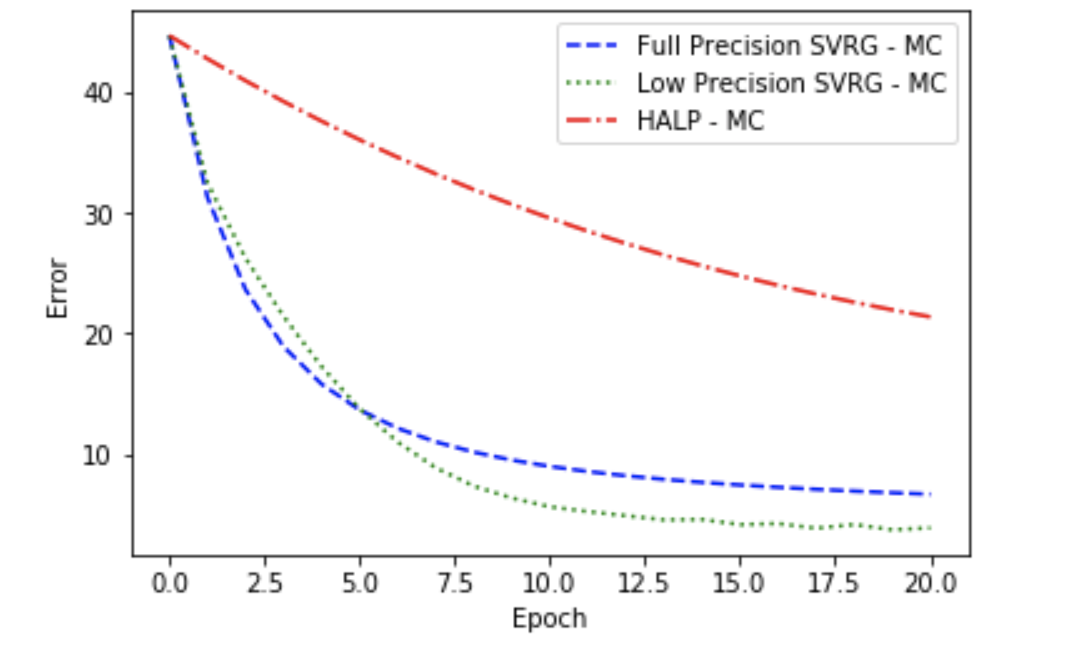
\includegraphics[width=.5\textwidth]{pic4.png}
    \caption{Comparison of algorithms epoch length of 200}
\end{figure}

\begin{figure}[ht!]
    \centering
    \includegraphics[width=.5\textwidth]{pic5.png}
    \caption{Comparison of algorithms epoch length of 100}
\end{figure}

\printbibliography



\end{document} 
